\subsection{Componentes}
\label{subsec:componentes}
% Motor: 
% https://www.pololu.com/product/2212
% https://www.pololu.com/product/2212
% Encoder:
% https://www.pololu.com/product/3081
% Driver motor:
% https://www.pololu.com/product/713
% ESP32:

São quatro o número de componentes básicos que compõem os robôs presentes neste trabalho, sendo eles: um par de atuadores (motor direito e esquerdo), um par de sensores de rotação (\textit{Encoders} magnéticos), um \emph{Driver} motor multicanal, um microcontrolador e bateria recarregável. Devido as características dos componentes escolhidos para o projeto, apenas estes quatro tipos foram suficiente para compor a eletrônica do robô de forma a respeitar as restrições dimensionais, realizar o controle dos motores de forma eficiência e com um bom período de amostragem e baixo gasto energético, além de um baixo custo financeiro. A seguir serão apresentados mais detalhes dos componentes supracitados.\\

\begin{figure}[H]
    \centering
    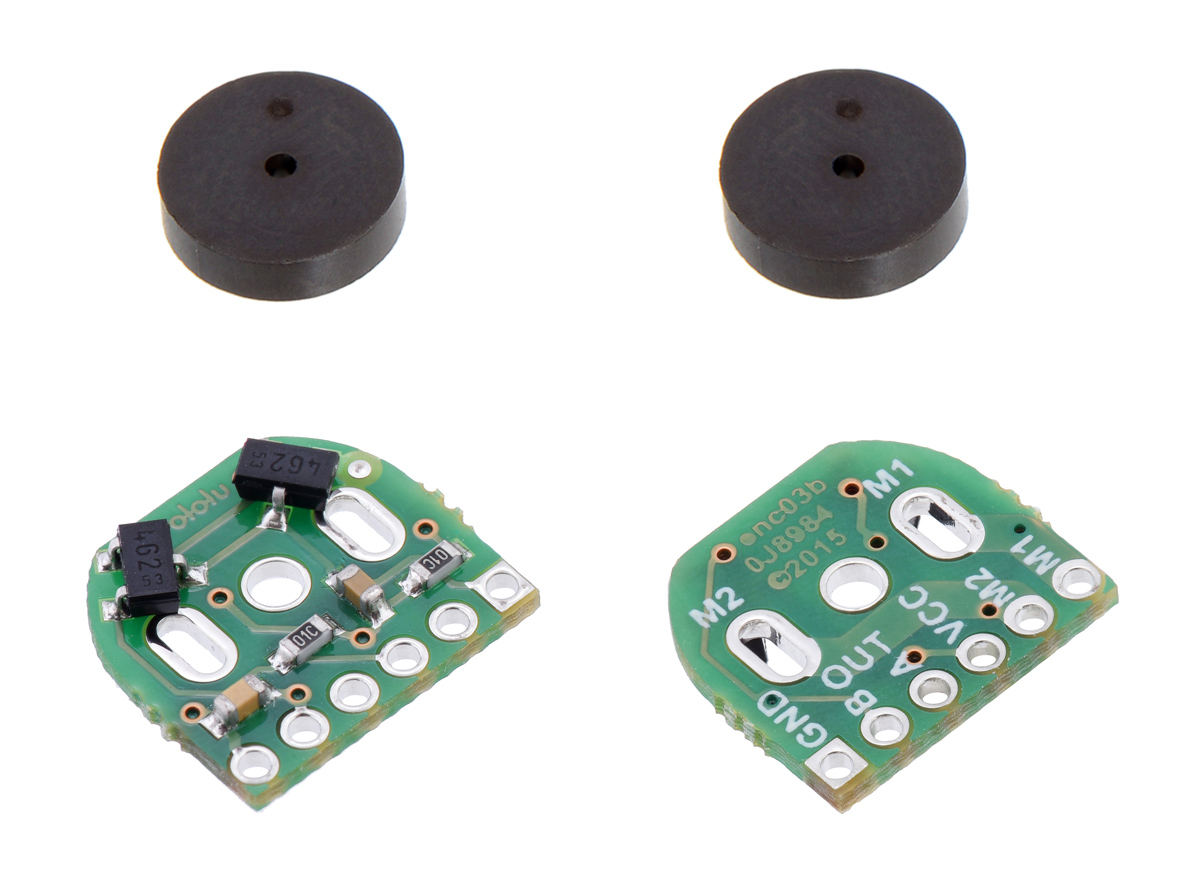
\includegraphics[width=5cm]{figuras/eletronica/encoder_frente_verso.jpg}
    \caption{Par de Encoders Magnéticos de até $12$ pulsos por revolução.}
    \label{fig:encoder}
    \fonte{\cite{Pololu:Encoder}.}
\end{figure}

Os sensores utilizados são \emph{Encoders} rotativos magnéticos do tipo incremental (ver Figura \ref{fig:encoder}). Eles podem ser trabalhados com uma resolução de até $12$ pulsos por revolução (se utilizado todas as bordas dos pulsos gerados). Esses sensores operam com uma faixa de tensão de alimentação de $2.7$V até $18$V.\\

% 30:1 Micro Metal Gearmotor HP 6V with Extended Motor Shaft
\begin{figure}[H]
    \centering
    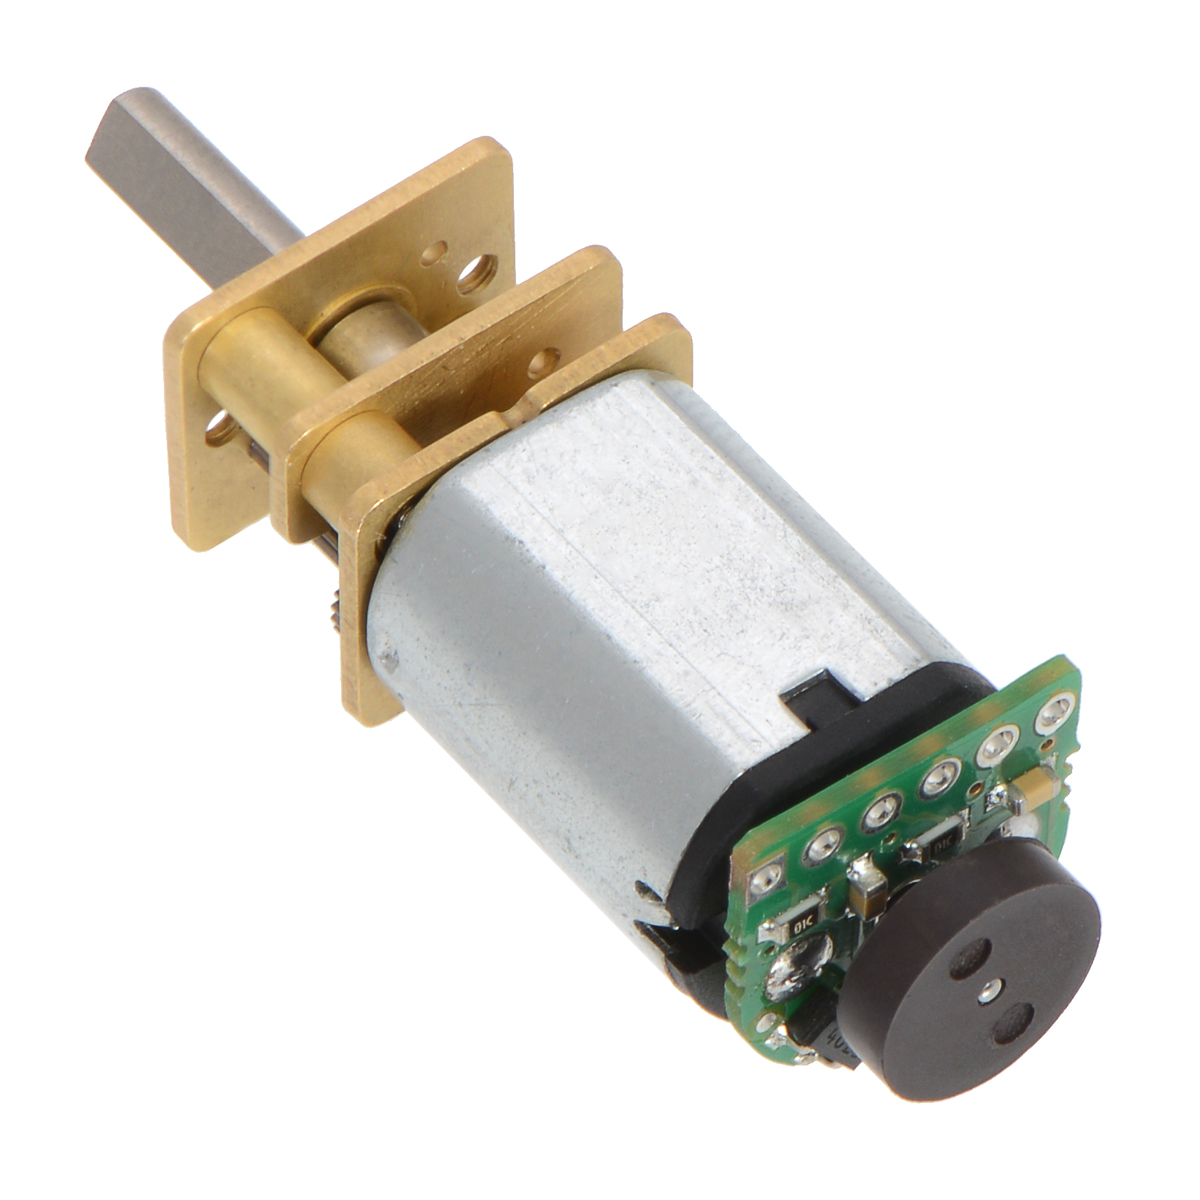
\includegraphics[width=3cm]{figuras/eletronica/motor_com_encoder.jpg}
    \caption{Micro Motor de 6V com caixa de redução de 30:1 e \textit{Encoder} magnético.}
    \label{fig:motor_com_encoder}
    \fonte{\cite{Pololu:Encoder_no_motor}.}
\end{figure}

A Figura \ref{fig:motor_com_encoder} mostra o motor escolhido equipado com o \textit{Encoder} magnético colocado em seu eixo estendido (placa de circuito impresso com um Imã natural em forma de disco), esse é um micro motor de $6$V com uma caixa de redução de $\approx 30:1$ da \textit{Pololu}\cite{Pololu}. A caixa de redução faz com que a resolução do sensor seja $30$ vezes maior no eixo do motor, ou seja, de uma resolução (máxima) de $12$PPR passa a gerar até o equivalente a $360$ pulsos por revolução.\\

\begin{figure}[H]
    \centering
    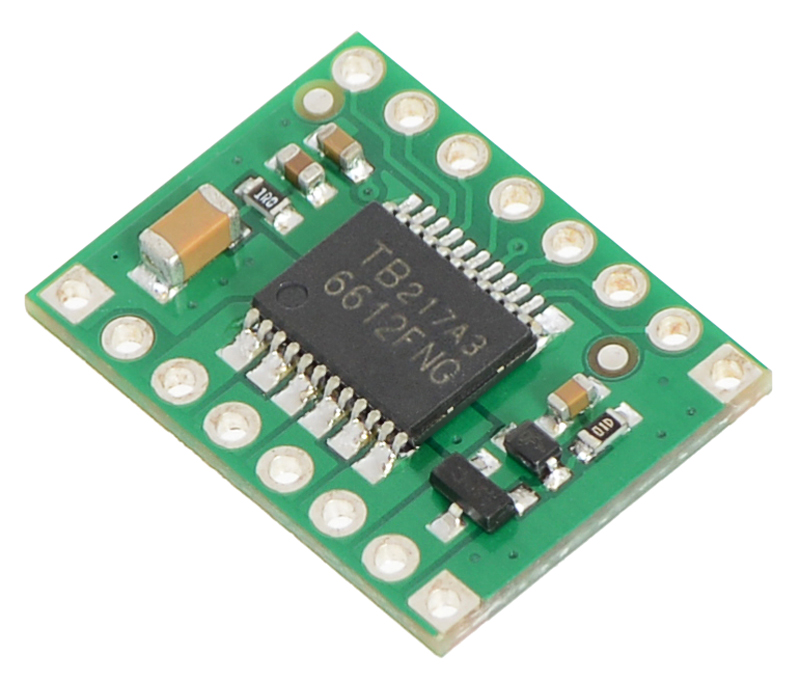
\includegraphics[width=3cm]{figuras/eletronica/driver.jpg}
    \caption{\textit{Driver} Motor TB6612FNG.}
    \label{fig:driver_motor}
    \fonte{\cite{Pololu:Driver}.}
\end{figure}

A Figura \ref{fig:driver_motor} mostra o \emph{Driver motor} utilizado. Ele é responsável por fazer o interfaceamento entre o $\mu{}C$ e os motores para garantir a separação dos circuitos de alta potência (motores) da de baixa ($\mu{}C$). O \emph{Driver} possui dois canais de controle de motores, ou seja, possui dois conjuntos de saídas de alta potência (até $3$A e $13.5$V) e dois de entrada para sinal PWM (frequência máxima de $100$ kHz, tensão lógica máxima de $5.5$V) para controlar dois motores separadamente. Além disso ele possui circuitos de proteção e proteção contra correntes inversas que possam ser geradas pelos motores.\\


\begin{figure}[H]
    \centering
    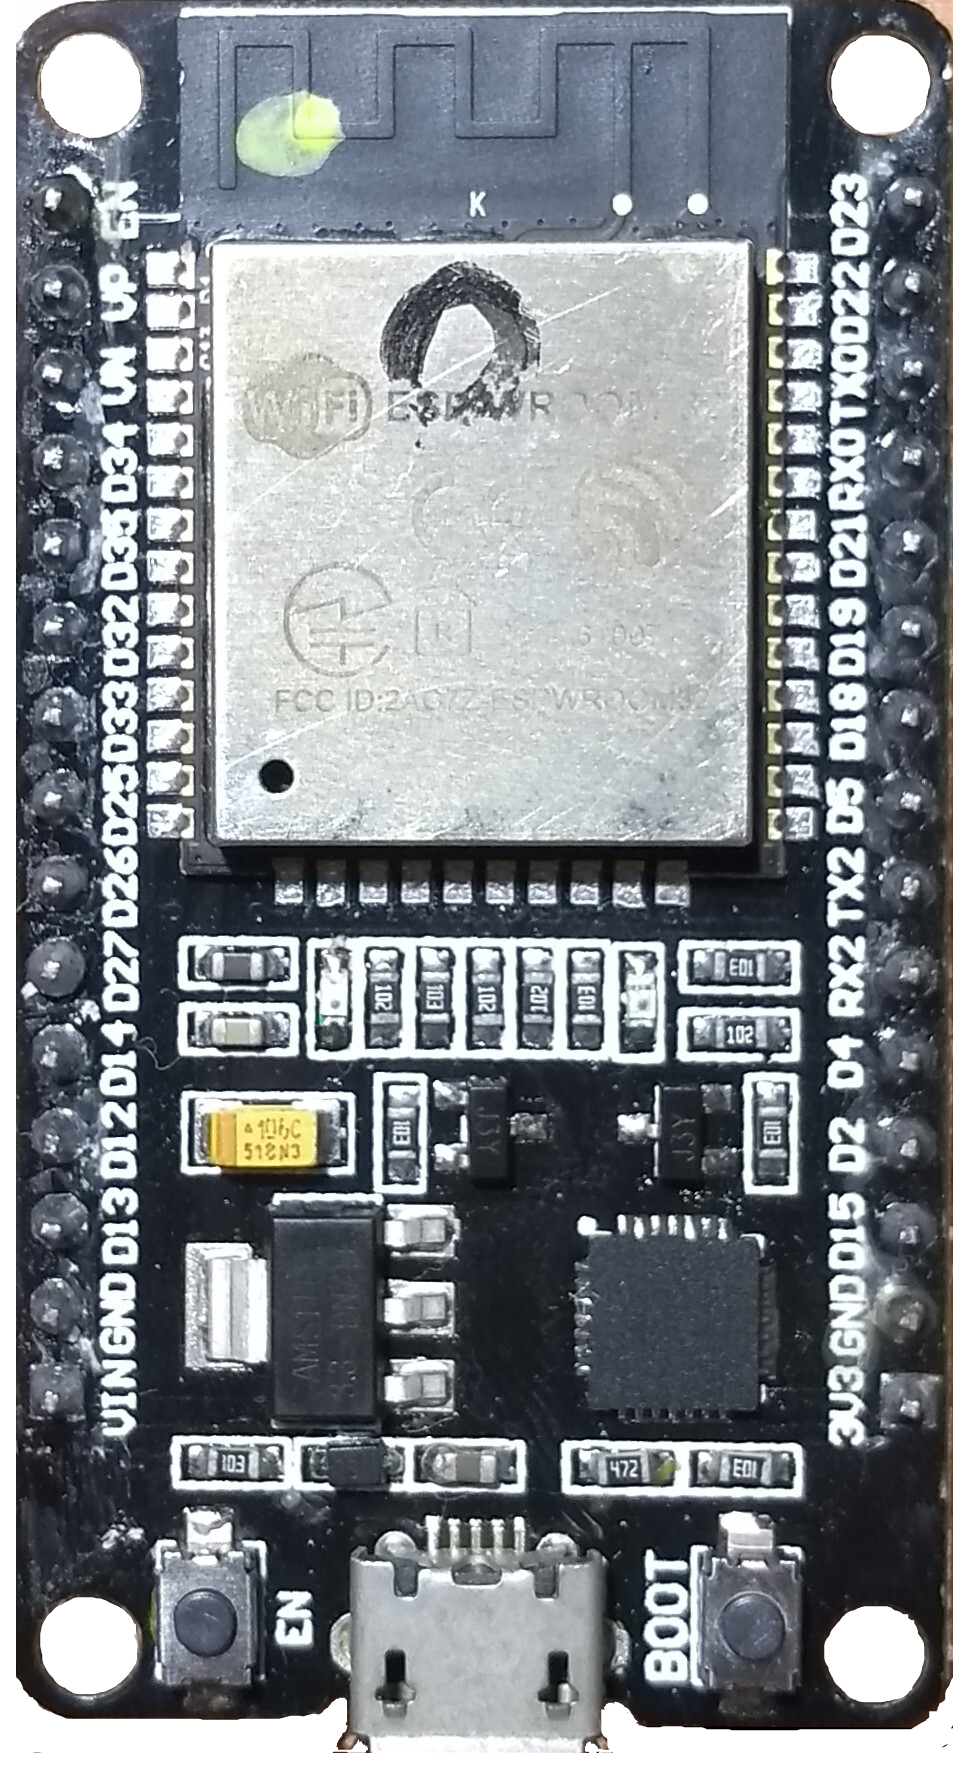
\includegraphics[width=3cm]{figuras/eletronica/esp32_kit.png}
    \caption{Placa de desenvolvimento ESP32 Dev1.}
    \fonte{Própria.}
    \label{fig:esp32_kit}
\end{figure}

O $\mu{}C$ utilizado foi o \emph{ESP32} da empresa \emph{Espressif Systems} em um \emph{kit} de desenvolvimento rápido (ver Figura \ref{fig:esp32_kit}). O microcontrolador possui um microprocessador \emph{Tensilica Xtensa LX6} de $32$\emph{bits} com as seguintes especificações \cite{esp32:datasheet}:

\begin{itemize}
    \item CPUs: 2 núcleos principais e um terceiro núcleo de baixo consumo enérgico. 
    \item Frequência do \emph{clock} dos núcleos: Até $240$ MHz
    \item Desempenho: $600$ DMPIS
    \item Interface \emph{Wireless}: Wi-Fi: 802.11 b/g/n/e/i (802.11n @ 2.4 GHz até 150 Mbit/s), Bluetooth: v4.2 BR/EDR e Bluetooth Low Energy (BLE).
    \item Memória: 448 Kb de ROM e 520 Kb de SRAM.
\end{itemize}


\begin{figure}[H]
    \centering
    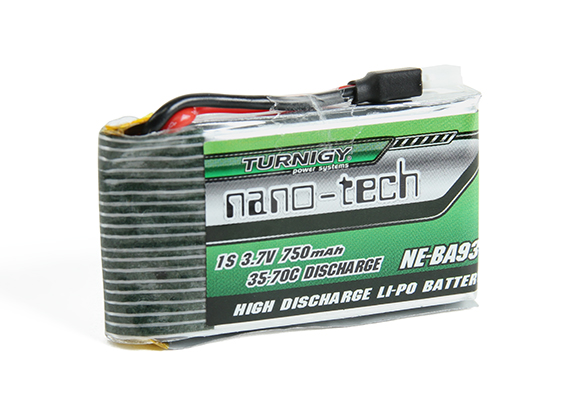
\includegraphics[width=0.5\textwidth]{figuras/eletronica/bateria.jpg}
    \caption{Bateria Lipo 1s 3.7v 750mah Ne-ba931.}
    \label{fig:bateria_lipo}
    \fonte{\cite{bateria:futuramix}.}
\end{figure}

A Figura \ref{fig:bateria_lipo} apresenta a bateria utilizada. É uma bateria de 1 célula (1S), portanto, de $3.7$V e com uma capacidade de carga de $750$mAh.
